% !TEX root=../../Thesis.tex
\chapter{Introduction} \label{ch:intro}
The way we transport ourselves is currently evolving, and \gls{ad} technology is expected to have a big impact on this transformation~\cite{traffic21, McKinsey2023}. With \gls{av} the efficiency of traffic can be improved by scheduling commercial transports outside of rush hours~\cite{FAGNANT2015167}. Number of parking spots in cities can be reduced if the vehicles can autonomously drive itself to a less crowded area when not in use and drive back when needed. Congestion and traffic jams could also be reduced if a large amount of vehicles in traffic are autonomous and optimize around the same goal e.g., traffic flow or fuel efficiency. 

The rapid success of \gls{ml} during the last decades has lead to major progress towards deploying \gls{av}s in the real world. One clear benefactor of these new \gls{ml} technics are the perception systems~\cite{Janai2020}. Better perception enables more accurate representation of the environment. 
% The low-level control of the vehicle is a mature research area and can be solved with classical control theory methods~\cite{Paden2016}.
However, navigating complex scenarios such as urban intersections and roundabouts with dense traffic remain challenging for \gls{av}s because it requires a higher level of interaction between road users, as summarized in a review paper~\cite{Schwarting2018}. 
When a human driver approach an intersection, they observe the environment to identify the traffic light, signs and other approaching vehicles. Then assess the situation to determine \textit{who has the right of way?} Before deciding weather to drive or yield. 
% If all drivers could perfectly assess the situation and follow the right of way, there would be no accidents or collisions between cars. 
% Despite, each year over one million people are killed in traffic-related accidents, where the vast majority of the accidents are caused by human mistakes~\cite{WHO2018, NHTSA2018}. 
But human drivers are not perfect, according to the Insurance Institute for Highway Safety~\cite{IIHS2019}, in 2019, an estimated \num{115741} people were injured by drivers running a red light, whereas \num{928} of them were killed. 
While these accidents were mainly caused by driver inattention or reckless driving, it motivates the development of decision-making algorithms for \gls{av}s which not only follow the traffic rules but can also take into account other drivers future actions and inattention, which is the main focus in this thesis. 
%\todo{Level 2: Volvo pilot assist and tesla auto pilot. Level 4: Waymo. Woven automated city}
% That is why this thesis will focus on intersection scenarios that includes interactions of other vehicles and propose a \gls{rl} approach using deep Q-learning while considering the uncertainty of . 

% This thesis presents a deep Q-learning approach for creating decision-making strategies for \gls{av}s driving in environments with other drivers without explicitly knowing their intentions. 
% Starting with introducing the different \gls{ad} levels in Section~\ref{sec:intro_ad}.
% Section~\ref{sec:intro_intersections} defines the terms' scenario, intersection and intention used in this thesis.
% \Citet{Shalev2016} raises two concerns when using \gls{ml}, especially Reinforcement learning, for autonomous driving applications: ensuring functional safety of the driving policy and solving the \gls{mdp} model is problematic, because of unpredictable behavior of other drivers. 
% Ensuring functional safety is not the main focus of this work, but because of its importance, it is briefly addressed in Section~\ref{sec:system_architecture} together with a proposed system architecture that can utilize the work presented in this thesis in a ''safe'' way. 
% The handling of the unpredictable behavior of other drivers is the main topic in this thesis and the research questions are presented in Section~\ref{sec:research_questions}. The scope and limitations are listed in Section~\ref{sec:scope}. Finally, the contributions of this thesis is presented in Section~\ref{sec:contributions}. 

\section{Autonomous Driving Levels}
\label{sec:intro_ad}
When talking about autonomous driving, it is first important to specify which level of autonomy that is being discussed. The Society of Automotive Engineers has classified these different levels of autonomy ranging from zero to five~\cite{SAE2021}, also referred to as L0-L5. The first level L0 is a vehicle with no autonomy, whereas a fully \gls{av} that can operate in any environment and without any human supervision is defined as L5. Popular \gls{adas} functions today, like lane centering or adaptive cruise control are classified as L1, while the Volvo Pilot Assist and Tesla Autopilot that provide both steering and acceleration/breaking are classified as level 2. The main criteria for L2 systems is that the driver is in control and only supported by the system. This puts a requirement on the driver to always supervise the vehicle and take over when needed to ensure safety. For L3 and higher the responsibility of driving is shifted to the system. At L3, the driver still has to take control over the vehicle but at only the request of the system, and at L4 and L5 the autonomous driving features no longer require the driver to take over. Finally, the main difference between L4 and L5 is the capability of driving anywhere, under all conditions. Examples of L4 are robot taxis developed by Waymo, Zoox, cruise and Toyota which only operate in a specified area or city. 

% Another way to categorize these autonomy levels is: supervised and unsupervised driving. Supervised driving include L0-L3 where the driver has to supervise the system and take control when necessary, while unsupervised 
% \tommy{Level 2: You are diving, provide steering and breaking support to the driver, lane centering and adaptive cruise control}

The \gls{av} making the decisions in this work are referred to as the ego vehicle, while other traffic participants are assumed to be vehicles driven by other human drivers but could be extended to pedestrians bicyclist and other \gls{av}s. 
The methods presented in this thesis are aimed at an autonomy level L5. At this level the system is expected to handle all aspects of driving within a specific task such as crossing an intersection. 

\subsection{Intersections, intention and scenarios}
\label{sec:intro_intersections}
When it comes to the scenarios considered in this work. This section aims to clearify the use of the words' intersection, intention and scenario.
% When a pedestrian approach a crossing they have been taught at a young age to look at both sides of the road before crossing. The same apply for a human driver approaching an intersection. 
% When a human driver approach an intersection, it is natural to observe the environment to identify the traffic light, signs and other approaching vehicles. Then assess the situation, who has the right of way? 

% The intention of the other driver can be guided by the 
% Recently nontraditional intersections are also becoming increasingly popular. The goal of these designs is to reduce the number and/or severity of conflict points by altering the customary vehicular paths at the intersection. In light of the increased focus on and occurrence of these intersection types, it is expected that the application of nontraditional designs will continue to spread.

\begin{figure}[h]
	\centering
	\begin{subfigure}[t]{0.48\columnwidth}
		\centering
		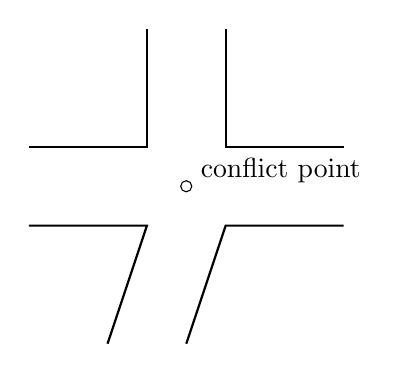
\begin{tikzpicture}
			% Crossing
			\def\crossleftx{-2}
			\def\crossrightx{2}
			\def\crosstopy{2}
			\def\crossboty{-2}
			\def\roadwidth{0.5}

			\draw (0,0) circle (2pt);
			\node at (1.2, 0.2) {conflict point};
			\draw[thick] (\crossleftx, \roadwidth) -- (-\roadwidth, \roadwidth) -- (-\roadwidth, \crosstopy);
			\draw[thick] (\crossleftx, -\roadwidth) -- (-\roadwidth, -\roadwidth) -- (-\roadwidth-\roadwidth, \crossboty);
			\draw[thick] (\roadwidth, \crosstopy) -- (\roadwidth, \roadwidth) -- (\crossrightx, \roadwidth);
			\draw[thick] (\roadwidth-\roadwidth, \crossboty) -- (\roadwidth, -\roadwidth) -- (\crossrightx, -\roadwidth);
		\end{tikzpicture}
		\caption{Single intersection}
\end{subfigure}%
	~ 
	\begin{subfigure}[t]{0.48\columnwidth}
		\centering
		\begin{tikzpicture}
			% Crossing
			\def\crossleftx{-2.5}
			\def\crossrightx{2.5}
			\def\crosstopy{2}
			\def\crossboty{-2}
			\def\roadwidth{0.5}

			\draw (-0.5,0) circle (2pt);
			\draw (0.5,0) circle (2pt);
			% \node at (0.7, 0.2) {crossing point$^1$};
			\draw[thick] (\crossleftx, \roadwidth) -- (-\roadwidth-0.5, \roadwidth) -- (-\roadwidth-0.5, \crosstopy);
			\draw[thick] (\crossleftx, -\roadwidth) -- (-\roadwidth-0.5, -\roadwidth) -- (-\roadwidth-0.5, \crossboty);
			\draw[thick] (0, \crosstopy) -- (0, \roadwidth);
			\draw[thick] (0, -\roadwidth) -- (0, \crossboty);
			\draw[thick] (\roadwidth+0.5, \crosstopy) -- (\roadwidth+0.5, \roadwidth) -- (\crossrightx, \roadwidth);
			\draw[thick] (\roadwidth+0.5, \crossboty) -- (\roadwidth+0.5, -\roadwidth) -- (\crossrightx, -\roadwidth);
		\end{tikzpicture}
		\caption{Double intersection}
	\end{subfigure}

	\caption{Examples of different intersections}
	\label{fig:example_intersections}

\end{figure}
An intersection refers the geometrical shape of the roads intersecting each other e.g., number of junctions, conflict points, turns and angle of incidence, as shown in Figure~\ref{fig:example_intersections}. 
An intersection can either be signalized or unsignalized, a signalized intersection has something to define the right-of-way e.g., a regulatory (i.e., STOP or YIELD) sign or a traffic signal, while an unsignalized intersection does not. But as mentioned in the introduction, humans do not always follow these right-of-way rules and therefore end up in accidents. That is why this thesis defines the intentions as what other vehicle will do in the future: stop, slow down or drive through the intersection. If the intention is known, then all intersections can be treated as unsignalized since the right-of-way can be implied by the intention instead of the infrastructure. This way, even when another vehicle would break a traffic rule and run a red light, a good agent would still stop and be safe. 
%  Intersections in the world often have something to decide the right of way like traffic rules, signs or lights. 
% While there exists a large variation of intersections in the world, this work only focus on the decision to drive or yield, we can reduce the dimention to 1. 

Finally, the combination of an intersection, its' traffic participants, their intentions, positions and velocities, is defined as a scenario shown in Figure~\ref{fig:example_scenarios}. 
More detail on the specific intersections and scenarios considered in this work is presented in Chapter~\ref{ch:modeling_intersection}.

\begin{figure}[h]
	\centering
	\begin{subfigure}[t]{0.48\columnwidth}
		\centering
		\begin{tikzpicture}
			% Crossing
			\def\crossleftx{-2}
			\def\crossrightx{2}
			\def\crosstopy{2}
			\def\crossboty{-2}
			\def\roadwidth{0.5}

			\draw (0,0) circle (2pt);
			% \node at (1.2, 0.2) {crossing point};
			\draw[thick] (\crossleftx, \roadwidth) -- (-\roadwidth, \roadwidth) -- (-\roadwidth, \crosstopy);
			\draw[thick] (\crossleftx, -\roadwidth) -- (-\roadwidth, -\roadwidth) -- (-\roadwidth, \crossboty);
			\draw[thick] (\roadwidth, \crosstopy) -- (\roadwidth, \roadwidth) -- (\crossrightx, \roadwidth);
			\draw[thick] (\roadwidth, \crossboty) -- (\roadwidth, -\roadwidth) -- (\crossrightx, -\roadwidth);

			% 	cars
			\node[inner sep=0pt] (ego_car) at (\crossleftx+0.5,0)
			{\includegraphics[width=.18\textwidth, angle=0]{figures/ego_car_top_down.png}};

			\node[inner sep=0pt] (target_car) at (0,\crosstopy-0.5)
			{\includegraphics[width=.18\textwidth, angle=-90]{figures/target_car_top_down.png}};

			%  \node[inner sep=0pt] (targetcar2) at (0,2.5)
			%  {\includegraphics[width=.18\textwidth, angle=-90]{figures/target_car_top_down.png}};
			%  \node (tctext2) [right=of targetcar2] {Car 2};
			
			% \node[inner sep=0pt] (target_car_1) at (0,-1.5)
			% {\includegraphics[width=.18\textwidth, angle=-90]{figures/target_car_top_down.png}};
			% \node (tc_text1) [right=of target_car_1] {Car 1};
		\end{tikzpicture}
		\caption{Single intersection scenario}
\end{subfigure}%
	~ 
	\begin{subfigure}[t]{0.48\columnwidth}
		\centering
		\begin{tikzpicture}
			% Crossing
			\def\crossleftx{-2.5}
			\def\crossrightx{2.5}
			\def\crosstopy{2}
			\def\crossboty{-2}
			\def\roadwidth{0.5}

			\draw (-0.5,0) circle (2pt);
			\draw (0.5,0) circle (2pt);
			% \node at (0.7, 0.2) {crossing point$^1$};
			\draw[thick] (\crossleftx, \roadwidth) -- (-\roadwidth-0.5, \roadwidth) -- (-\roadwidth-0.5, \crosstopy);
			\draw[thick] (\crossleftx, -\roadwidth) -- (-\roadwidth-0.5, -\roadwidth) -- (-\roadwidth-0.5, \crossboty);
			\draw[thick] (0, \crosstopy) -- (0, \roadwidth);
			\draw[thick] (0, -\roadwidth) -- (0, \crossboty);
			\draw[thick] (\roadwidth+0.5, \crosstopy) -- (\roadwidth+0.5, \roadwidth) -- (\crossrightx, \roadwidth);
			\draw[thick] (\roadwidth+0.5, \crossboty) -- (\roadwidth+0.5, -\roadwidth) -- (\crossrightx, -\roadwidth);

			% 	cars
			\node[inner sep=0pt] (ego_car) at (\crossleftx+0.5,0)
			{\includegraphics[width=.18\textwidth, angle=0]{figures/ego_car_top_down.png}};

			\node[inner sep=0pt] (target_car) at (-0.5,\crosstopy-0.5)
			{\includegraphics[width=.18\textwidth, angle=-90]{figures/target_car_top_down.png}};

			\node[inner sep=0pt] (target_car_2) at (0.5,\crossboty+0.5)
			{\includegraphics[width=.18\textwidth, angle=90]{figures/target_car_top_down.png}};
		\end{tikzpicture}
		\caption{Double intersection scenario}
	\end{subfigure}

	\caption{Examples of different scenarios}
	\label{fig:example_scenarios}

\end{figure}

\tommy{what I want to say here is: define an unsignalized intersection. There are many variations. Roundabouts are defined as unsignalized intersection. To satisfy the requirement of being able to drive anywhere for level 5 it is necessary to find a method that can scale to these different scenarios}

%  In light of the increased focus on and occurrence of these intersection types nationwide, it is expected that the application of nontraditional designs will continue to spread.



\section{Research questions}
\label{sec:research_questions}
% This thesis defines human driving as sequential decision making under uncertainty. Decisions such as overtaking a slow driver or when to cross an intersection are often made with limited information and some prediction estimate based on previous experience. 
% This section briefly introduce the intersection problem, why its hard and the research questions that are studied in this paper. 
% % A simple unsignalized intersection is shown in Figure \ref{fig:zones}.
% In some cases like highway driving the uncertainty is very low, but when it comes to more urban environment this uncertainty increases. Compared to highway, urban environments introduce more uncertainty. 
% Investigate how \gls{rl} methods can be used in practice to create a tactical decision making agent for \gls{ad}.

% \tommy{This paper focus on the DQN algorithm and investigate how far we can push it for decision making}

% \begin{enumerate}
% 	\item The goal for the ego vehicle is to drive through intersections without colliding. 
% 	\item The intersection can be of different shapes. %We assume we have a map of the intersection. 
% 	\item There will be other vehicles crossing the same intersection. 
% 	\item The intention of other drivers are not known
	
% \end{enumerate}

The work presented in this thesis investigate the following research questions:
\begin{enumerate}
	\item[\textbf{Q1.}] How can \gls{rl} be used to create a decision-making agent for driving through intersections? (PAPER A and B)
	\item[\textbf{Q2.}] In what way can an \gls{rl} agent utilize the uncertainty of its predictions and actions? (PAPER C and D)
	\item[\textbf{Q3.}] How do can a \gls{rl} agent handle situations it has not been trained on? (PAPER C and E)
	
	% \item[\textbf{Q3.}] How can the quality of a RL agent be improved by accounting for uncertainty? (PAPER C and D)
	% \item[\textbf{Q1.}] How can RL be used to create a decision-making agent for autonomous driving, that can handle different unsignalized intersections (complex urban scenarios)? Learn a scalable policy that is able to handle different scenarios. Relative coordinate system. Action space. 
	% (specificera for att komma undan varfor har du inte kollat pa andra metoder. How can we use RL for AD )
	% \item[\textbf{Q2.}] Can a good driving policy be found without explicitly predicting other drivers intentions?
	% \item[\textbf{Q2.}] Can we find a driving policy without explicitly predicting other drivers intentions?
	% LSTM or other netowrk structures can find the hidden state that is intention. 
	% \item[\textbf{Q3.}] How can MPC be used to improve the action and state space for a RL agent? 
	% \item[\textbf{Q3.}] How do we model the actions to drive through an intersection as discreet? (PAPER A and B)
	% \item[\textbf{Q3.}] How can AD domain knowledge (and models) be used to improve the action and state space for a RL agent? MPC for actions, Particle filter for intention distribution. How can AD domain knowledge be used to create a state and action space that improves the RL agent?
	% (How can the uncertainty of the RL agent be utilized?) (RPF-in the output and PF-in the input space)
	% \item[\textbf{Q5.}] Where does ML/RL fit in the system architecure for decision making?
	% (PAPER A shows that RL can make decisions that finds a gap inbetween cars, PAPER B found that we RL can learn the utility of different actions and decrease the computational power required by modeling and predicting each action in the MPC. While MPC can ganerate a safe path that guarantees safety.) 
\end{enumerate}

\section{Scope and limitations}
\label{sec:scope}
The following aspects of creating a tactical decision making agent for autonomous driving in uncertain environments are not considered in this thesis. 

\begin{enumerate}
	% \item We have access to sensors on-board the ego vehicle. We do not have v2v, or v2x communication. 
	% \item We do not assume any knowledge of traffic signs or traffic lights. 
	\item Do not guarantee safety, the best we can do its making the decisions not trigger collision avoidance functions. 
	\item The work in this thesis is tested in simulation environments and not real world. 
	\item This work considers the control of one vehicle and not multiple agents. 
	% \item This work considers the control of one vehicle and not multiple agents. 
	% \item A reward function is defined for each approach. 
	
	% To compensate for not having v2v or v2x communication, we have to, directly or indirectly, predict what other driver will do. 
	
\end{enumerate}


\section{Contributions}
\label{sec:contributions}
\todo{Rewrite once thesis is in a better state}
The main contributions of this thesis are:
\begin{enumerate}
	\item a \gls{pomdp} formulation for driving in intersections. 
	\item A neural network architecture that is invariant to permutations of the order of which surrounding traffic participants are observed, which speeds up training and improves the quality of the trained agent. 
	\item REWRITE: A belief state representation using a particle filter and a comparison and analysis of different algorithms that utilize the belief state. 
	\item Two approached to solving a POMDP with hidden intention state. LSTM layer and belief state. 
	% \item General state space representation that is invariat to permutations of the intersection design. 
	\item Extension of \gls{rl} methods that provide an estimate of the epistemic uncertainty and use it to create a confidence criteria that can identify situations with high uncertainty. 
	\item Method for choosing between a set of fully trained policies. 

\end{enumerate}


\section{Thesis outline}
\todo{rewrite when thesis is more finished}
The outline of the thesis is as follows: in Chapter \ref{ch:related_work} other research in the same field is presented. In Chapter \ref{ch:background} introduce the mathematical framework \gls{mdp} and \gls{pomdp} with a brief theory of \gls{rl}. 
Chapter \ref{ch:modeling_intersection} is where the problem is formulated by defining the components of the \gls{pomdp}. In Chapter \ref{ch:mpc}, performance results from using deep Q-learning to solve the \gls{pomdp} is presented and later combined with a \gls{mpc} to improve the actions. Later in Chapter \ref{ch:uncertainty} two approaches to handle the uncertainty is presented. First the uncertainty in the decisions from the \gls{rl} algorithm and then an empirical study of how well a \gls{dqn} can handle uncertainty of others driving intentions. Chapter \ref{ch:generalize} present an approach to generalize over differnt \gls{mdp}s more specifically policies learned from different transfer functions. 


